\documentclass[mathserif,notes]{beamer}
\usepackage{mybeamertheme}
\usepackage{pdfsync} % works only on TeXShop, comment otherwise
\usepackage{pgf}
\usepackage{multimedia} % to embed movies in the PDF file
\usepackage{xcolor}
\usepackage{graphicx}
\usepackage{comment}
\usepackage{pgfpages}
\usepackage{topcapt}
\usepackage{booktabs}

% for the tikz pictures
\usepackage{geometry}
\geometry{hmargin=1cm,vmargin=1cm}
\usepackage{tikz}
\def\width{5}
\def\hauteur{5}

\mode<presentation>
{
  \usetheme{Madrid}   %  \usetheme{Warsaw}
  % Note: this next command makes nice slides, but Adobe doesn't like it (you get blank pages)
  %\setbeamertemplate{background canvas}[vertical shading][bottom=white,top=structure.fg!15]
  \setbeamertemplate{footline}{\pgfuseimage{UCM-logo}}

  %\usecolortheme{seahorse}
  \usecolortheme{beaver}
 % \setbeamercovered{transparent}
}
%\usepackage[T1]{fontenc}
% For printing purposes only
%\pgfpagesuselayout{4 on 1}[letterpaper,border shrink=5mm,landscape]

\usepackage{amssymb,amsmath}
\hypersetup{%
 pdftitle={Math298 Lecture 4},
 pdfauthor={Juan Meza(UC Merced)},
 pdfsubject={Fundamental Concepts in Computational and Applied Mathematics},
 pdfkeywords={linear algebra, sparse, iterative}
 }
 
\title[Math 298]{Math 298 \\
Fundamental Concepts in \\ Computational and Applied Mathematics}  \subtitle{Lecture 4}
\author[Juan Meza]{Juan Meza \\ School of Natural Sciences \\ University of California, Merced}
\date[September 30, 2013]{}
\institute[UC Merced]

\pgfdeclareimage[height=0.35cm]{UCM-logo}{UCM-logo}
\pgfdeclareimage[width=0.8\textwidth]{Hurricane}{Hurricane}
\pgfdeclareimage[width=0.5\textwidth]{Uniform}{ParaView_UG_Uniform}
\pgfdeclareimage[width=0.5\textwidth]{Curve}{ParaView_UG_Curvilinear}
\pgfdeclareimage[width=0.5\textwidth]{Rect}{ParaView_UG_Rectilinear}
\pgfdeclareimage[width=0.5\textwidth]{AMR}{ParaView_UG_AMR}
% \logo{\pgfuseimage{UCM-logo}}

%% figures






% Common abbreviations
% (Remember to put '\ ' after if an interword space is
%  desired rather than end-of-sentence space. Same for '.etc)' ).
\newcommand{\eg}{{\em e.g.}}		% e.g.
\newcommand{\ie}{{\em i.e.}}		% i.e.
\newcommand{\etc}{{\em etc.}}		% etc.
\newcommand{\vs}{{\em vs.}}		% vs.
\newcommand{\remark}{{\color{red} Remark:} }


\newcommand {\DS} {\displaystyle}
\newcommand{\eref}[1]{{\rm{(\ref{#1})}}}
\newcommand{\tref}[1]{{\rm{\ref{#1}}}}


\def\frechet{Fr\'echet\ }
\def\more{Mor\'e\ }
\def\fl{{\sf fl}}
\def\flop{{\sf flop} }
\def\flops{{\sf flops} }
\def\matlab{{\sc Matlab} }
\def\Matlab{\matlab}

\def\bigO{\mathcal{O}}

% Mathematical Symbols

\newcommand{\deq}{\raisebox{0pt}[1ex][0pt]{$\stackrel{\scriptscriptstyle{\rm def}}{{}={}}$}}

\newcommand {\half} {\mbox{$\frac{1}{2}$}}  %machine epsilon
\newcommand{\set}[2]{\left\{ #1 \;:\; #2 \right\}}

\newcommand {\macheps} {\mathbf{\epsilon}}  %machine epsilon
\newcommand {\real} {\mathbb{R}}
\newcommand {\nat} {\mathbb{N}}
\newcommand {\compl} {\mathbb{C}}
\newcommand {\diag} {{\mbox{diag}}}
\newcommand {\meas} {{\mbox{meas}}}
\newcommand {\mspan} {{\mbox{span}}}

\newcommand {\pdx} {\frac{\partial}{\partial x}}
\newcommand {\pdt} {\frac{\partial}{\partial t}}
\newcommand {\pdxx} {\frac{\partial^2}{\partial x^2}}
\newcommand {\dx} {\frac{d}{d x}}
\newcommand {\dt} {\frac{d}{d t}}
\newcommand {\dxx} {\frac{d^2}{d x^2}}

\newcommand {\bA} {\mbox{\boldmath $A$}}
\newcommand {\bB} {\mbox{\boldmath $B$}}
\newcommand {\bF} {\mbox{\boldmath $F$}}
\newcommand {\bI} {\mbox{\boldmath $I$}}
\newcommand {\bP} {\mbox{\boldmath $P$}}
\newcommand {\bY} {\mbox{\boldmath $Y$}}
\newcommand {\bZ} {\mbox{\boldmath $Z$}}
\newcommand {\ba} {\mbox{\boldmath $a$}}
\newcommand {\bb} {\mbox{\boldmath $b$}}
\newcommand {\bd} {\mbox{\boldmath $d$}}
\newcommand {\bff}{\mbox{\boldmath $f$}}
\newcommand {\bk} {\mbox{\boldmath $k$}}
\newcommand {\bp} {\mbox{\boldmath $p$}}
\newcommand {\bs} {\mbox{\boldmath $s$}}
\newcommand {\bu} {\mbox{\boldmath $u$}}
\newcommand {\bv} {\mbox{\boldmath $v$}}
\newcommand {\bw} {\mbox{\boldmath $w$}}
\newcommand {\bx} {\mbox{\boldmath $x$}}
\newcommand {\by} {\mbox{\boldmath $y$}}
\newcommand {\bz} {\mbox{\boldmath $z$}}
\newcommand {\blambda} {\mbox{\boldmath $\lambda$}}
\newcommand {\btau} {\mbox{\boldmath $\tau$}}

%
% JCM Quantum Chemistry commands
%
\newcommand{\bra}[1]{\langle #1|}
\newcommand{\ket}[1]{|#1\rangle}
\newcommand{\braket}[2]{\langle #1|#2\rangle}
% Example of usage
%\[
%\ket{\Psi}=\sum_{i}\ket{\phi_i}\braket{\phi_i}{\Psi}
%\]

%
% Other symbols
%
\newcommand {\grad}{\nabla}
\newcommand {\hess}{\nabla^2}
\newcommand {\condA}{\kappa(A)}

\newtheorem{algorithm}{Algorithm}

%

% \boxfig{pos}{wid}{text}:  A figure with a box around it
%
% pos	the usual figure placement arg: eg. htbp
% wid	the width of the figure, in some units: eg. 5in
% text	the contents of the figure, including picture/caption/label/etc
%
\newlength{\boxwidth}
\newcommand{\boxfigure}[3]{
	\begin{figure}[#1]
		\setlength{\boxwidth}{#2}
		\addtolength{\boxwidth}{.1in}

		\centering
		\framebox[\boxwidth]{
			\begin{minipage}{#2}
			#3
			\end{minipage}
		}
	\end{figure}  
}

% use \fullboxwidth for arg 2 of boxfigure to get box of size \textwidth


% \boxalg{pos}{text}:  An algorithm with a box around it
%
% title  the name of the algorithm
% text   the contents of the figure, including picture/caption/label/etc
%
\newcommand{\boxalg}[2]{
            \setlength{\boxwidth}{\fullboxwidth}
            \addtolength{\boxwidth}{.1in}
            \vspace{2ex}
            \framebox[\boxwidth][#1]{
                    \vspace{1ex}
                    \begin{minipage}{\fullinboxwidth}
                        #2
                    \end{minipage}
                    \vspace{1ex}
            }
            \vspace{2ex}
}






% see above
\newlength{\fullboxwidth}
\setlength{\fullboxwidth}{\textwidth}
\addtolength{\fullboxwidth}{-0.5in}

\newlength{\fullinboxwidth}
\setlength{\fullinboxwidth}{\fullboxwidth}
\addtolength{\fullinboxwidth}{-0.5in}






\definecolor{navy}{RGB}{0,0,128}
\definecolor{forestgreen}{RGB}{34,139,34}
\definecolor{mylightsteelblue}{RGB}{176,196,222}
\definecolor{mylightcyan}{RGB}{180,255,255}
\definecolor{mypaleturquoise}{RGB}{175,238,238}
\definecolor{mylightgoldenrod}{RGB}{250,250,210}
\definecolor{mylightyellow}{RGB}{255,255,224}
\definecolor{mylightsalmon}{RGB}{255,160,122}

\setbeamercolor{blacklightsteelblue}{fg=black,bg=mylightsteelblue}
\setbeamercolor{blackpaleturquoise}{fg=black,bg=mypaleturquoise}
\setbeamercolor{blacklightcyan}{fg=black,bg=mylightcyan}
\setbeamercolor{blacklightgoldenrod}{fg=black,bg=mylightgoldenrod}
\setbeamercolor{blacklightyellow}{fg=black,bg=mylightyellow}
\setbeamercolor{blacklightsalmon}{fg=black,bg=mylightsalmon}
\setbeamercolor{blackcyan}{fg=black,bg=cyan}




\begin{document}

%%%%%%%%%%%%%%%%%%%%%%%%%%%%%%%%%%%%%%%%%%%%%
\frame{

\titlepage

} % end frame

\section{Introduction}
%%%%%%%%%%%%%%%%%%%%%%%%%%%%%%%%%%%%%%%%%%%%%
\frame{\frametitle{Structured Grids}

\begin{itemize}
\item Some terminology
\begin{itemize}
\item cells, elements; triangles, quads, tetrahedrons, hex
\item node, vertex
\item edge, face
\end{itemize}

\item Properties
\begin{itemize}
\item quality of mesh
\item degeneracy
\item dof
\end{itemize}

\end{itemize}
} % end frame

%%%%%%%%%%%%%%%%%%%%%%%%%%%%%%%%%%%%%%%%%%%%%
\frame{\frametitle{Structured Grid Examples}

\begin{columns}[t]
\column{.5\textwidth}
Uniform Grid
\begin{itemize}
\item Simplest of all structured grids, $(i,j,k)$ indexing
\item Easy formula determining location of all nodes
\item What are the advantages/disadvantages?
\end{itemize}	
\column{.5\textwidth}
		\pgfputat{\pgfxy(0.0,-4.0)}{\pgfbox[left,base]{\pgfuseimage{Uniform}}}
\end{columns}
} % end frame

%%%%%%%%%%%%%%%%%%%%%%%%%%%%%%%%%%%%%%%%%%%%%
\frame{\frametitle{Structured Grid Examples}

\begin{columns}[t]
\column{.5\textwidth}
Rectilinear Grid
\begin{itemize}
\item Similar to uniform grid
\item What is the main advantage here?
\item What are the disadvantages?
\end{itemize}	
\column{.5\textwidth}
		\pgfputat{\pgfxy(0.0,-4.0)}{\pgfbox[left,base]{\pgfuseimage{Rect}}}
\end{columns}

} % end frame

%%%%%%%%%%%%%%%%%%%%%%%%%%%%%%%%%%%%%%%%%%%%%
\frame{\frametitle{Structured Grid Examples}


\begin{columns}[t]
\column{.5\textwidth}
Curvilinear Grid
\begin{itemize}
\item Note that each node still has the same number of neighbors
\item What is the main advantage here?
\item What are the disadvantages?
\end{itemize}	
\column{.5\textwidth}
	\pgfputat{\pgfxy(0.0,-4.0)}{\pgfbox[left,base]{\pgfuseimage{Curve}}}
\end{columns}



} % end frame

%%%%%%%%%%%%%%%%%%%%%%%%%%%%%%%%%%%%%%%%%%%%%
\frame{\frametitle{Structured Grid Examples}

\begin{columns}[t]
\column{.5\textwidth}
Adaptive Mesh Refinement Grid
\begin{itemize}
\item Block structured
\item Solves problem of having too much resolution in places that you don't need it
\item Software is more complicated
\item Error analysis more difficult
\end{itemize}	
\column{.5\textwidth}
	\pgfputat{\pgfxy(0.0,-4.0)}{\pgfbox[left,base]{\pgfuseimage{AMR}}}
\end{columns}

} % end frame

\section{SIM}
%%%%%%%%%%%%%%%%%%%%%%%%%%%%%%%%%%%%%%%%%%%%%
\frame{\frametitle{Properties of Structured Grids}

\begin{itemize}

\item Number of adjacent mesh elements is always the same
\item Generally more accurate per dof
\item Convergence of algorithms (linear solvers) usually faster
\item Better data layout, which is good for computation
\end{itemize}

} % end frame

%%%%%%%%%%%%%%%%%%%%%%%%%%%%%%%%%%%%%%%%%%%%%
\frame{\frametitle{5-Point Stencil}

\begin{columns}[c]
\begin{column}{.4\textwidth}
5-point stencil
\begin{itemize}
\item Simplest 2-D case
\item Leads directly to a sparse (penta-diagonal) matrix
\item Easy to solve with iterative methods
\end{itemize}
\end{column}

\begin{column}{.6\textwidth}
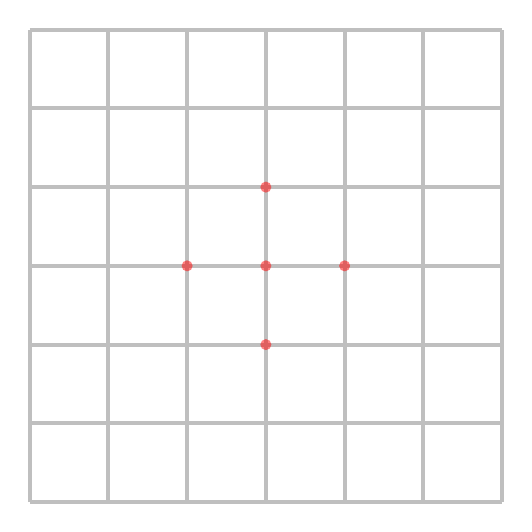
\begin{tikzpicture}[x=1cm, y=1cm, semitransparent]
%\draw[step=1mm, line width=0.1mm, black!30!white] (0,0) grid (\width,\hauteur);
%\draw[step=5mm, line width=0.2mm, black!40!white] (0,0) grid (\width,\hauteur);
%\draw[step=5cm, line width=0.5mm, black!50!white] (0,0) grid (\width,\hauteur);
\draw[step=1cm, line width=0.5mm, black!50!white] (-1,-1) grid (\width,\hauteur);
    \coordinate (u0) at (2,2);
    \coordinate (u1) at (2,1);
    \coordinate (u2) at (1,2);
    \coordinate (u3) at (3,2);
    \coordinate (u4) at (2,3);
    \fill[red] (u0) circle (2pt);
    \fill[red] (u1) circle (2pt);
    \fill[red] (u2) circle (2pt);
    \fill[red] (u3) circle (2pt);
    \fill[red] (u4) circle (2pt);
\end{tikzpicture}
\end{column}
\end{columns}

} % end frame

%%%%%%%%%%%%%%%%%%%%%%%%%%%%%%%%%%%%%%%%%%%%%
\frame{\frametitle{Intersecting lines}


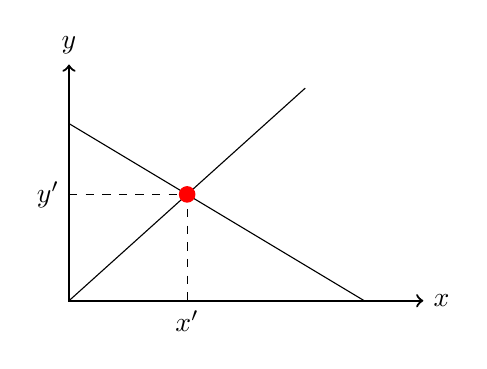
\begin{tikzpicture}[scale=1.5]
    % Draw axes
    \draw [<->,thick] (0,2) node (yaxis) [above] {$y$}
        |- (3,0) node (xaxis) [right] {$x$};
    % Draw two intersecting lines
    \draw (0,0) coordinate (a_1) -- (2,1.8) coordinate (a_2);
    \draw (0,1.5) coordinate (b_1) -- (2.5,0) coordinate (b_2);
    % Calculate the intersection of the lines a_1 -- a_2 and b_1 -- b_2
    % and store the coordinate in c.
    \coordinate (c) at (intersection of a_1--a_2 and b_1--b_2);
    % Draw lines indicating intersection with y and x axis. Here we use
    % the perpendicular coordinate system
    \draw[dashed] (yaxis |- c) node[left] {$y'$}
        -| (xaxis -| c) node[below] {$x'$};
    % Draw a dot to indicate intersection point
    \fill[red] (c) circle (2pt);
\end{tikzpicture}

} % end frame


\section{Applications}
%%%%%%%%%%%%%%%%%%%%%%%%%%%%%%%%%%%%%%%%%%%%%
\frame{\frametitle{Structured Grid Applications: Climate Modeling}

\pgfputat{\pgfxy(0.0,-4.0)}{\pgfbox[left,base]{\pgfuseimage{Hurricane}}}

} % end frame

\section{Summary}
%%%%%%%%%%%%%%%%%%%%%%%%%%%%%%%%%%%%%%%%%%%%%
\frame{\frametitle{Summary}

\begin{itemize}
\item Structured grids exist in many shapes and forms
\item Well developed and well understood methods available
\item Work extremely well on parallel and other high performance computing environments
\end{itemize}

}% end frame

%%%%%%%%%%%%%%%%%%%%%%%%%%%%%%%%%%%%%%%%%%%%%
\frame{\frametitle{References}

\begin{itemize}
\item {\bf Methods of Conjugate Gradients for Solving Linear Systems}, Magnus R. Hestenes and Eduard Stiefel, J. Res. of NBS, Vol. 49, No. 6, Dec. 1952.
\item {\bf Matrix Computations, 3rd Ed.}, Gene H. Golub and Charles F. Van Loan, Johns Hopkins, 1996.
\item {\bf Iterative Methods for Linear and Nonlinear Equations}, C.T. Kelley, SIAM,  1995.
\end{itemize}

}% end frame

\end{document}
